\documentclass{assignment}
\usepackage[pdftex]{graphicx} 
\usepackage{xcolor}
\definecolor{LightGray}{gray}{0.95}
%\usepackage{fancyvrb, minted} 
\usepackage[a4paper, margin = 2.5cm]{geometry} 
\usepackage[T1]{fontenc} 
% set figure path 
\graphicspath{figures}

\usepackage{amsmath, amsfonts, amssymb} 
\usepackage{hyperref, url}  
\usepackage{fancyhdr}
\usepackage{setspace}
\onehalfspacing

\usepackage{subcaption}


\student{Ahmet Akman 2442366}                             
\semester{Spring 2024}                            
\date{\today}                                   

\courselabel{EE449}          
\exercisesheet{Homework 1}{Report}  

\school{Middle East Technical University}        
\university{Electrical and Electronics Engineering}        

%%%%%%%%%%%%%%%%%%%%%%%%%%%%%%%%%%%%%%%%%%-DOCUMENT-%%%%%%%%%%%%%%%%%%%%%%%%%%%%%%%%%%%%%%%%%%%%

\begin{document}


\section{Question 1}

\subsection{Question 1.1 - Preliminaries}
The partial derivaive calculation steps for Tanh, Sigmoid and ReLU activation functions are shown in Figure \ref{partial_der}.
\begin{figure}[htbp!]
    \centering
    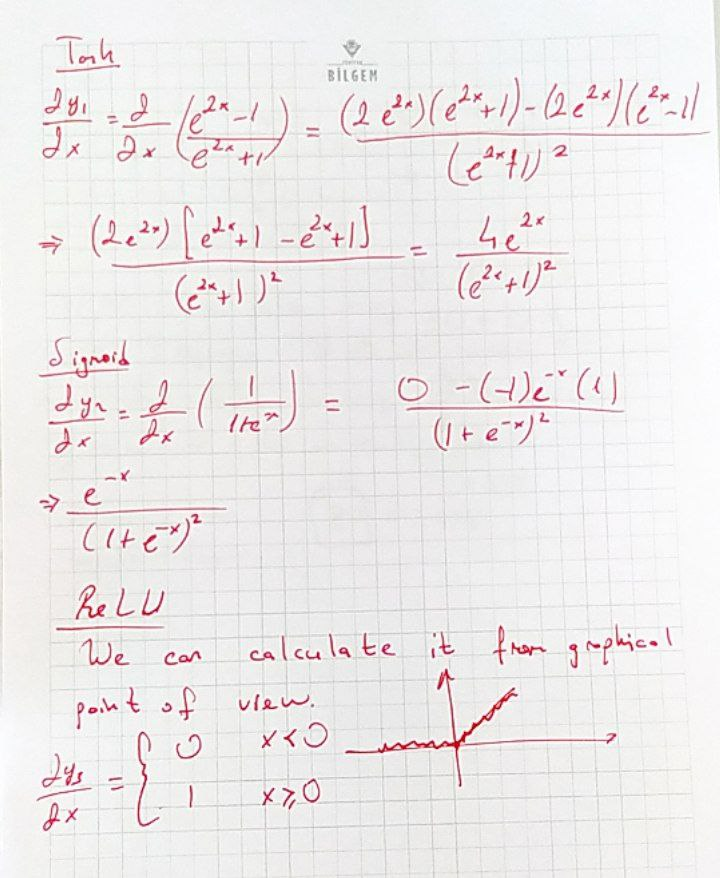
\includegraphics[width=0.6\textwidth]{figures/partial_der.jpg}
    \caption{Partial derivative calculation steps for Tanh, Sigmoid and ReLU activation functions.}
    \label{partial_der}
\end{figure}

Figure \ref{fig:activation_functions} illustrates the activation functions' response between -2 and 2. The plots are obtained using matplotlib library as instucted.

\begin{figure}[htbp!]
    \centering
    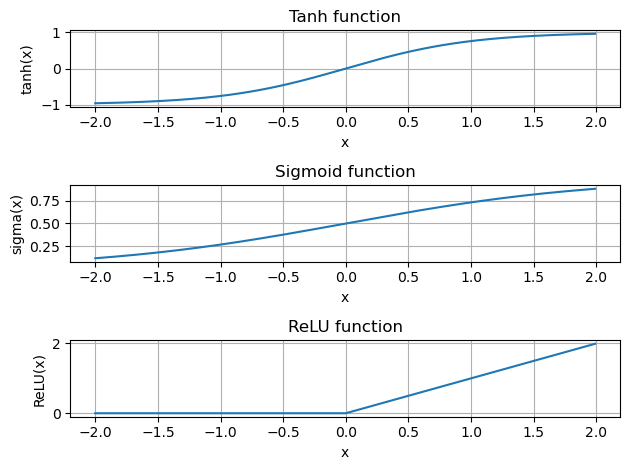
\includegraphics[width=1\textwidth]{figures/q1_1.png}
    \caption{Activation functions plot.}
    \label{fig:activation_functions}
\end{figure}

Figure \ref{fig:activation_functions_gradient} indicates the gradients of those functions in the same range. The gradients are calculated using the partial derivatives derived in Figure \ref{partial_der}.

\begin{figure}[htbp!]
    \centering
    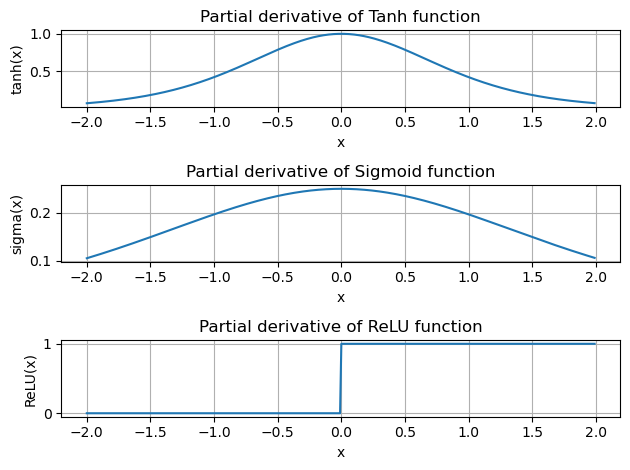
\includegraphics[width=1\textwidth]{figures/q1_2.png}
    \caption{Gradients of the activation functions plot.}
    \label{fig:activation_functions_gradient}
\end{figure}



\subsection{Question 1.2}

In this part, utilizing the given template of code, MLP with one hidden layer is implemented. The input-output pairs are fetched from the XOR data provided in utils.py. Note that for all networks learning rate is fixed to 0.00001 and seed is utilized. Figure \ref{fig:sigmoid_q1} shows the decision boundary for the sigmoid activated network. 
\begin{figure}[htbp!]
    \centering
    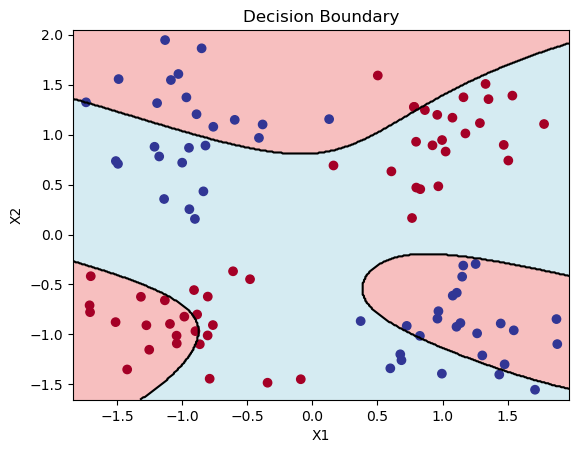
\includegraphics[width=1\textwidth]{figures/q1_sigmoid.png}
    \caption{Sigmoid activated XOR problem output.}
    \label{fig:sigmoid_q1}
\end{figure}
Similarly, Figure \ref{fig:tanh_q1} is the decision boundary for the tanh activated network and Figure \ref{fig:relu_q1} is the decision boundary for the ReLU activated network.


\begin{figure}[htbp!]
    \centering
    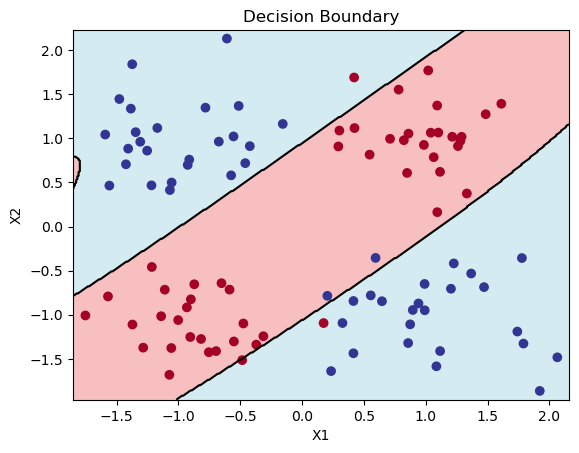
\includegraphics[width=1\textwidth]{figures/q1_tanh.png}
    \caption{Tanh activated XOR problem output.}
    \label{fig:tanh_q1}
\end{figure}

\begin{figure}[htbp!]
    \centering
    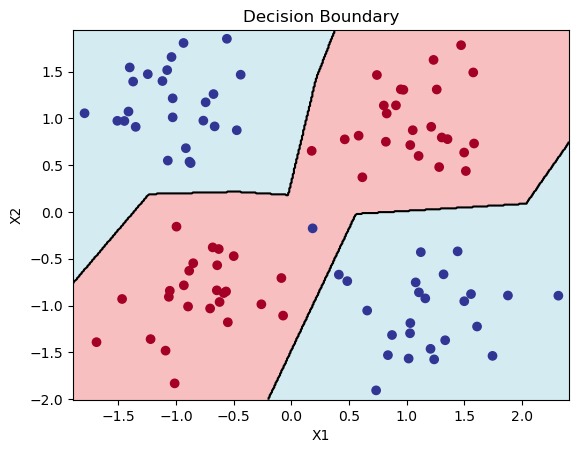
\includegraphics[width=1\textwidth]{figures/q1_relu.png}
    \caption{ReLU activated XOR problem output.}
    \label{fig:relu_q1}
\end{figure}

\subsection{Question 1.3}
\textbf{1.}
All of those activation functions provide a smooth transition from one state to another. The advantage of Tanh and Sigmoid is, they are limited in the range of -1 to 1 and 0 to 1, respectively. This property can be beneficial in some cases. However, the ReLU function is not limited in the range. It is also computationally cheaper than the other two. The disadvantage of ReLU is that it is not smooth at the origin. This can cause some problems in the optimization process. Another advantage of ReLU is negative gradients are zero. This may be helpful in some cases. 
\textbf{2.}

XOR problem is two input decision problem where inputs have to be different than each other to obtain 1. Since the output is always with respect to the state of two variables, decision boundary is not linear. Therefore, a single layer perceptron can not solve since in one step two case evaluations can not be done. Yet, by adding a hidden layer, the problem is solved. The activation functions are used to introduce non-linearity to the network. The decision boundary of the XOR problem is shown in Figures \ref{fig:sigmoid_q1}, \ref{fig:tanh_q1} and \ref{fig:relu_q1}. As can be seen from the figures, the MLP's with activation functions can solve the XOR problem at some extent.

\textbf{3.}
The boundaries change in each run, since the initial weights and the data points are randomly generated. Therefore, the decision boundaries are dependent on the training process where initial randomness lead to different outputs.


\section{Question 2}
A convolution operator is implemented using a set of nested loop. The outputs are checked on a seperate code so that they are identical to the output of torch.conv2d. Using the provided inputs, outputs provided in Figure \ref{fig:convolution_out} are obtained.

% 10 subfigure figure

\begin{figure}[htbp!]
    \begin{subfigure}{0.3\textwidth}
        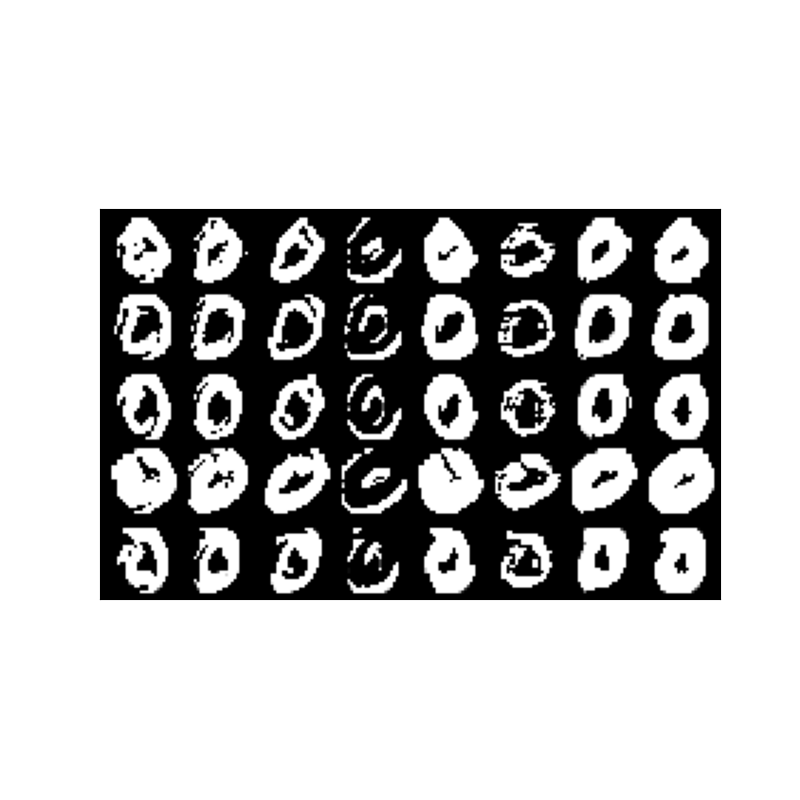
\includegraphics[width=\textwidth]{figures/out_0.png}
        \caption{Output 0}
    \end{subfigure}\hfill
    \begin{subfigure}{0.3\textwidth}
        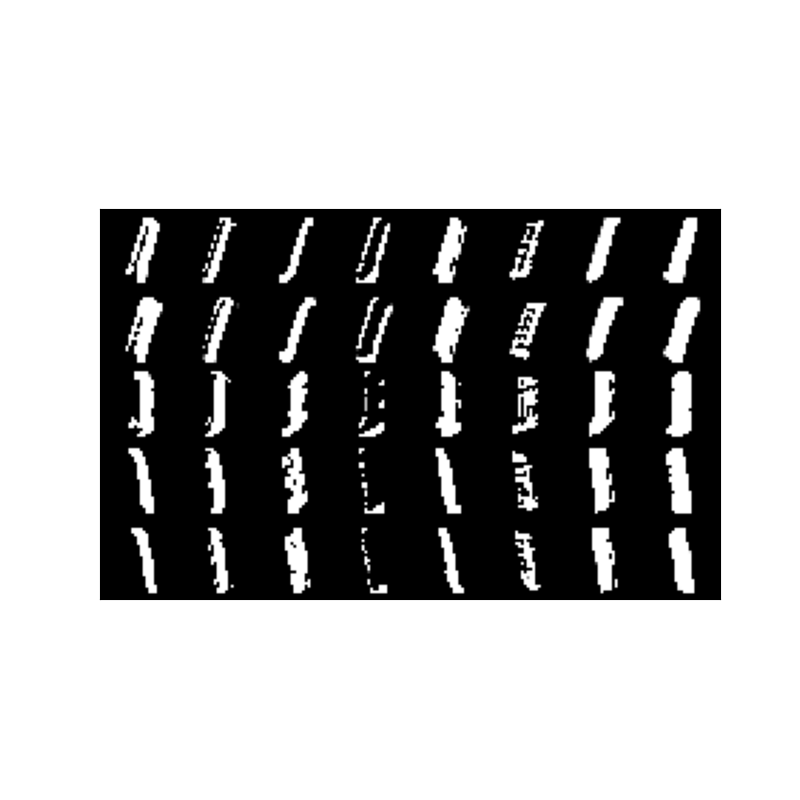
\includegraphics[width=\textwidth]{figures/out_1.png}
        \caption{Output 1}
    \end{subfigure}\hfill
    \begin{subfigure}{0.3\textwidth}
        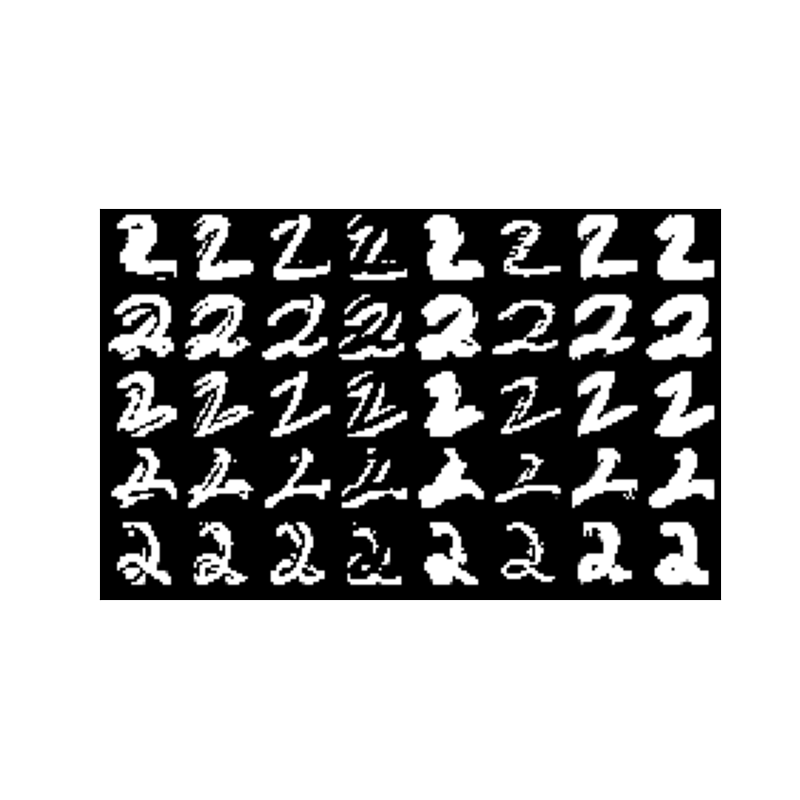
\includegraphics[width=\textwidth]{figures/out_2.png}
        \caption{Output 2}
    \end{subfigure}
    \vskip\baselineskip
    \begin{subfigure}{0.3\textwidth}
        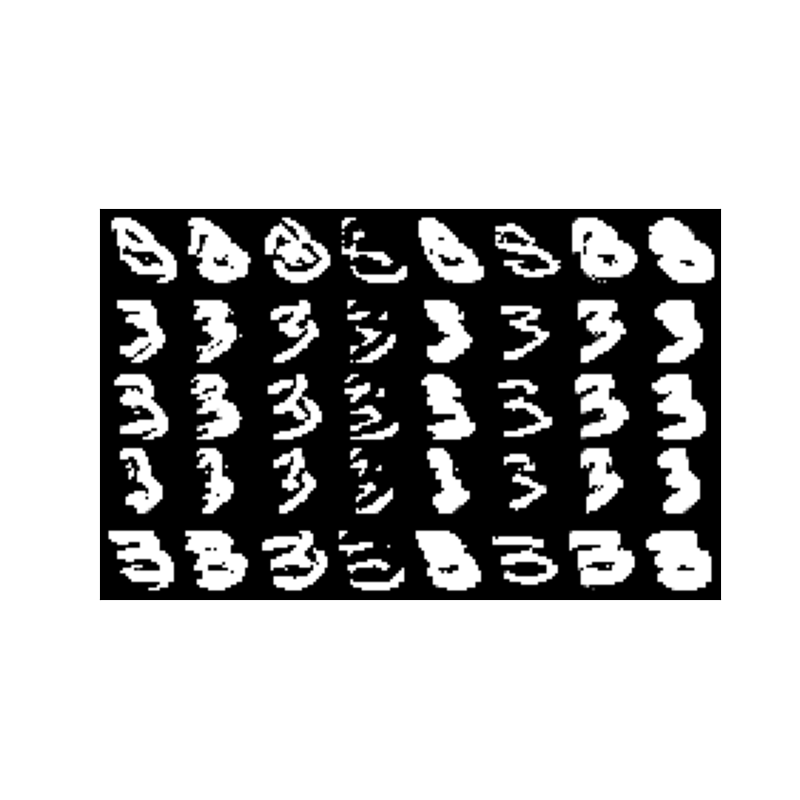
\includegraphics[width=\textwidth]{figures/out_3.png}
        \caption{Output 3}
    \end{subfigure}\hfill
    \begin{subfigure}{0.3\textwidth}
        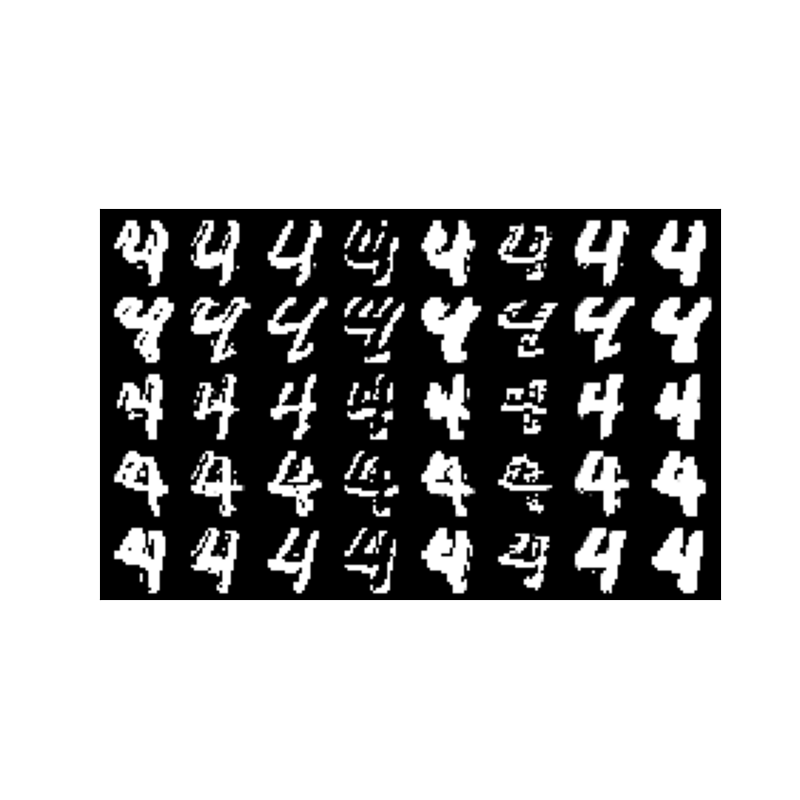
\includegraphics[width=\textwidth]{figures/out_4.png}
        \caption{Output 4}
    \end{subfigure}\hfill
    \begin{subfigure}{0.3\textwidth}
        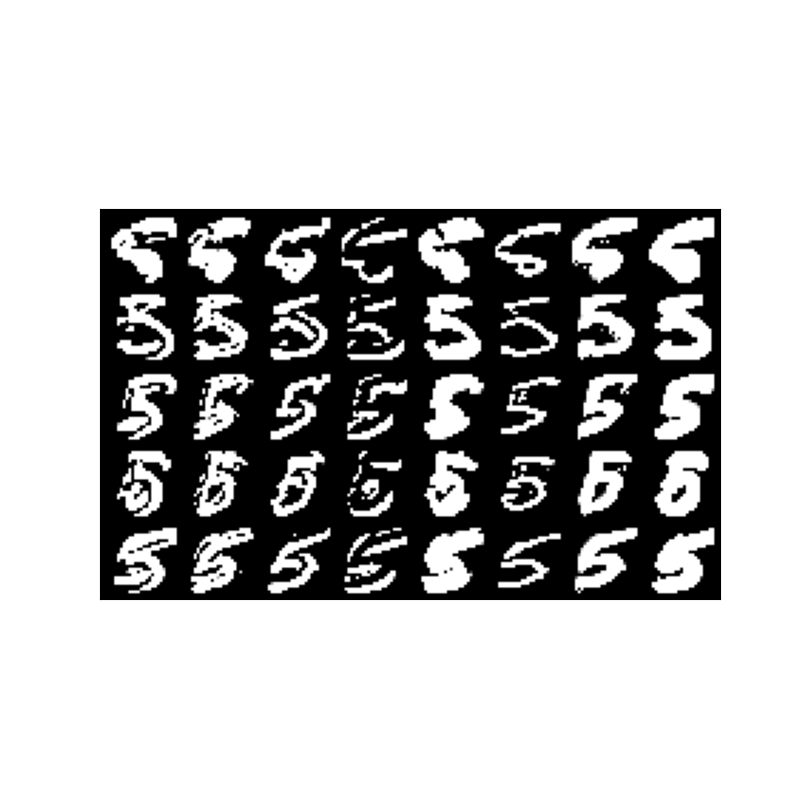
\includegraphics[width=\textwidth]{figures/out_5.png}
        \caption{Output 5}
    \end{subfigure}
    \vskip\baselineskip
    \begin{subfigure}{0.3\textwidth}
        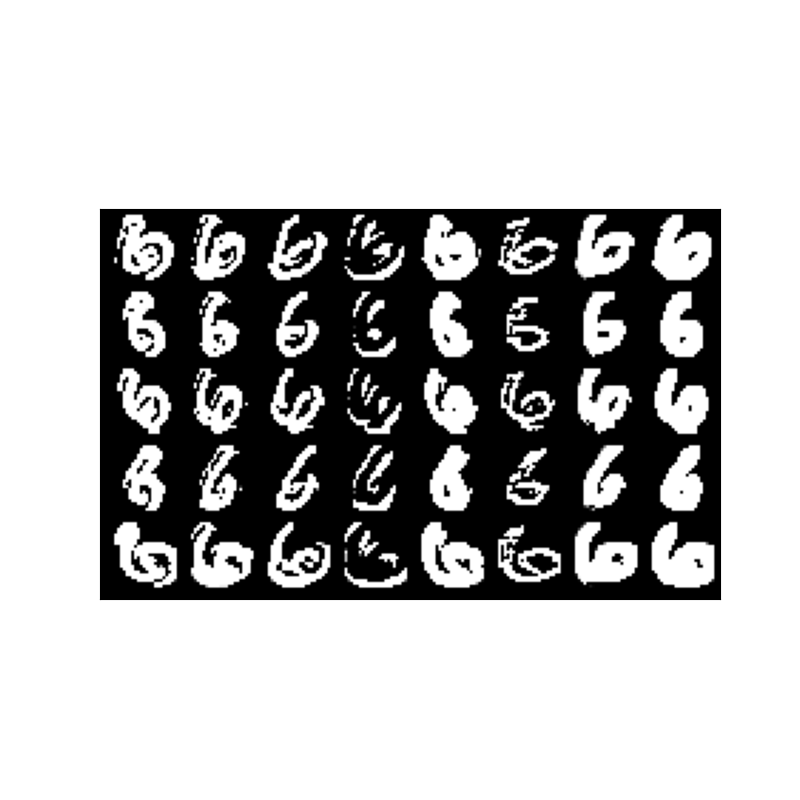
\includegraphics[width=\textwidth]{figures/out_6.png}
        \caption{Output 6}
    \end{subfigure}
    \hfill
    \begin{subfigure}{0.3\textwidth}
        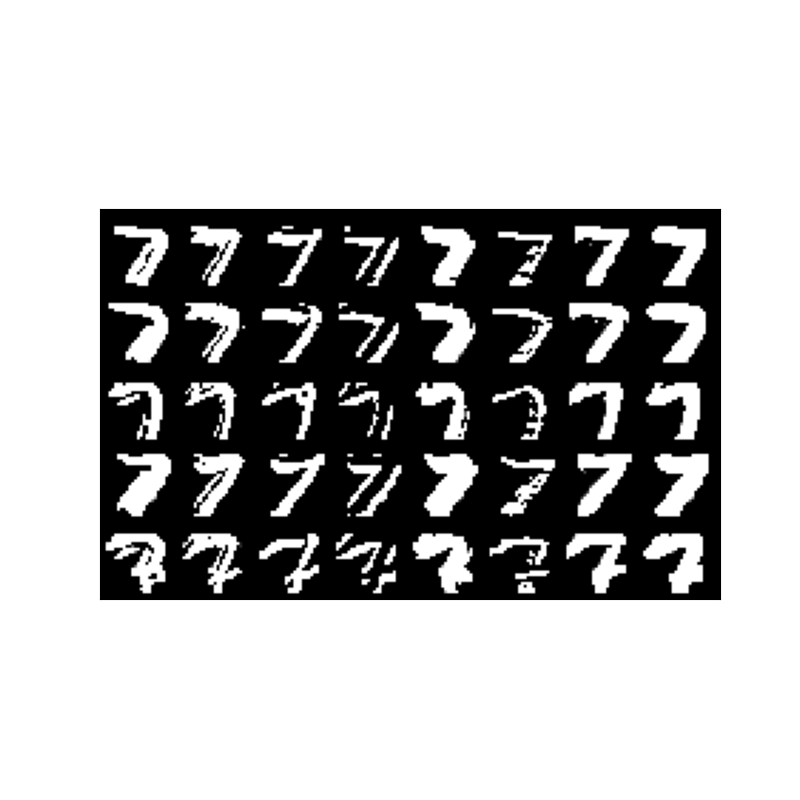
\includegraphics[width=\textwidth]{figures/out_7.png}
        \caption{Output 7}
    \end{subfigure}\hfill
    \begin{subfigure}{0.3\textwidth}
        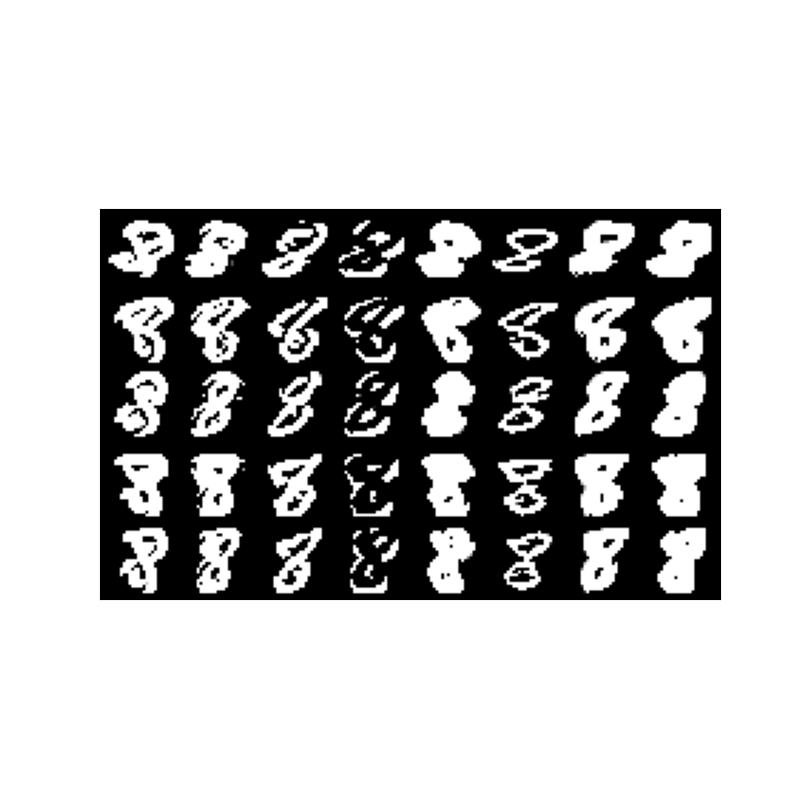
\includegraphics[width=\textwidth]{figures/out_8.png}
        \caption{Output 8}
    \end{subfigure}
    \vskip\baselineskip
    \begin{subfigure}{0.3\textwidth}
        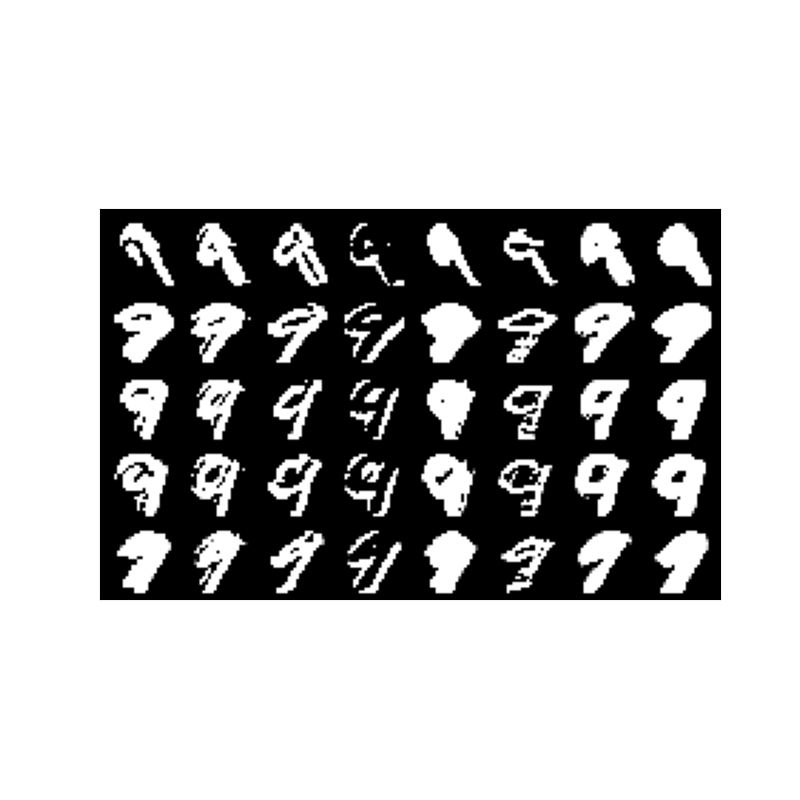
\includegraphics[width=\textwidth]{figures/out_9.png}
        
        \caption{Output 9}
    \end{subfigure}\hfill
    \caption{Convolution output}
    \label{fig:convolution_out}
\end{figure}
\subsection{Question 2.2 - Discussions}
\textbf{1.}
Two dimensional convolution operation provides filtering in two dimension via a kernel. The kernel is applied to the input image in a sliding window fashion. The output is obtained by element-wise multiplication of the kernel and the input image. The kernel is then shifted by a stride and the process is repeated. That is, two dimensional convolution operation with learnable kernal entries are commonly used in image processing to extract features from the image. The kernel is learned during the training process. Those feature maps encode necessary information about distinct clues in the image. For example in the case of object recognition, a specific kernel can be trained to detect bicyle rims. 
Kernel of a convolution layer corresponds to the filter function in one dimension. It is used to suppress or enhance certain information in the input image.

\textbf{2.}The sizes of the kernel corresponds to the size of the filter. Therefore, the size list can be explained as follows (batch size, input channels, output channels, filter height, filter width) . Batch size is the number of input sets in a batch if batching is used, here we have not utilized it. Input channels are the number of depth dimension in the image, for example in RGB frames it is three. This might be different for different sensor inputs and representations. The output channel number determines the depth dimension of the output tensor. The filter height and width are the dimensions of the filter.

\textbf{3.}
To understand what exactly happened here, let us plot the kernel and input for the number zero. Figure \ref{fig:kernel_input} illustrates the plot.

\begin{figure}[htbp!]
    \begin{subfigure}{0.5\textwidth}
        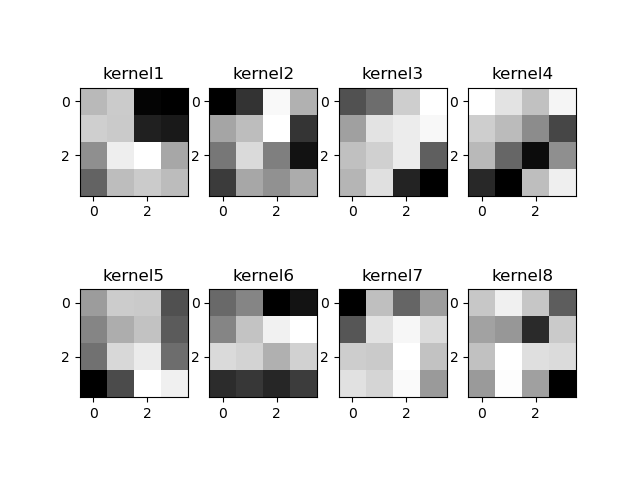
\includegraphics[width=\textwidth]{figures/q2_kernels.png}
        \caption{Kernels}
    \end{subfigure}\hfill
    \begin{subfigure}{0.5\textwidth}
        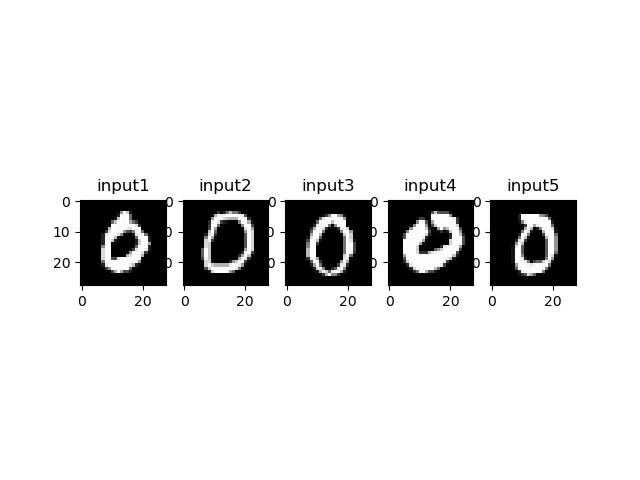
\includegraphics[width=\textwidth]{figures/q2_zero_input.png}
        \caption{Input set for number zero.}
    \end{subfigure}
    \caption{Kernel and input for number zero.}
    \label{fig:kernel_input}
\end{figure}
When we have a look at what output image represents, on each row an input image is convolved with a kernel. There are different kernels applied to the input image. The output image is the result of those convolutions. Figure \ref{fig:kernel_input} shows the input and kernel pairs in order.

\textbf{4.}
Each convolution kernel embeds a certain feature of the image. That is, if we have a look at Figure \ref{fig:kernel_input}.a we can see that kernel 4 enhances the countours on the image whereas kernel 6 enhances the filled part of those contours. This is the reason why we see similarly formatted outputs on the same column.
\textbf{5.}
Similarly, since we "highlight" different properties on the image with out filters, we see different patterns on the output side even if the input is the same.

\textbf{6.}
So, we can interpret form 4, and 5 that the output of the convolution layer is the result of the feature extraction process. The output is the result of the convolution of the input image with the learned filters. The output is the feature map that encodes the information about the input image. By post-processing those feature maps, we can obtain the necessary interpreations about the input image.

\section{Question 3}
\subsection{Question 3.1}
The implementations related to each architectures are completed as instructed. The code is given in appendix. As the result the plot shown in Figure 

\begin{figure}[htbp!]
    \centering
    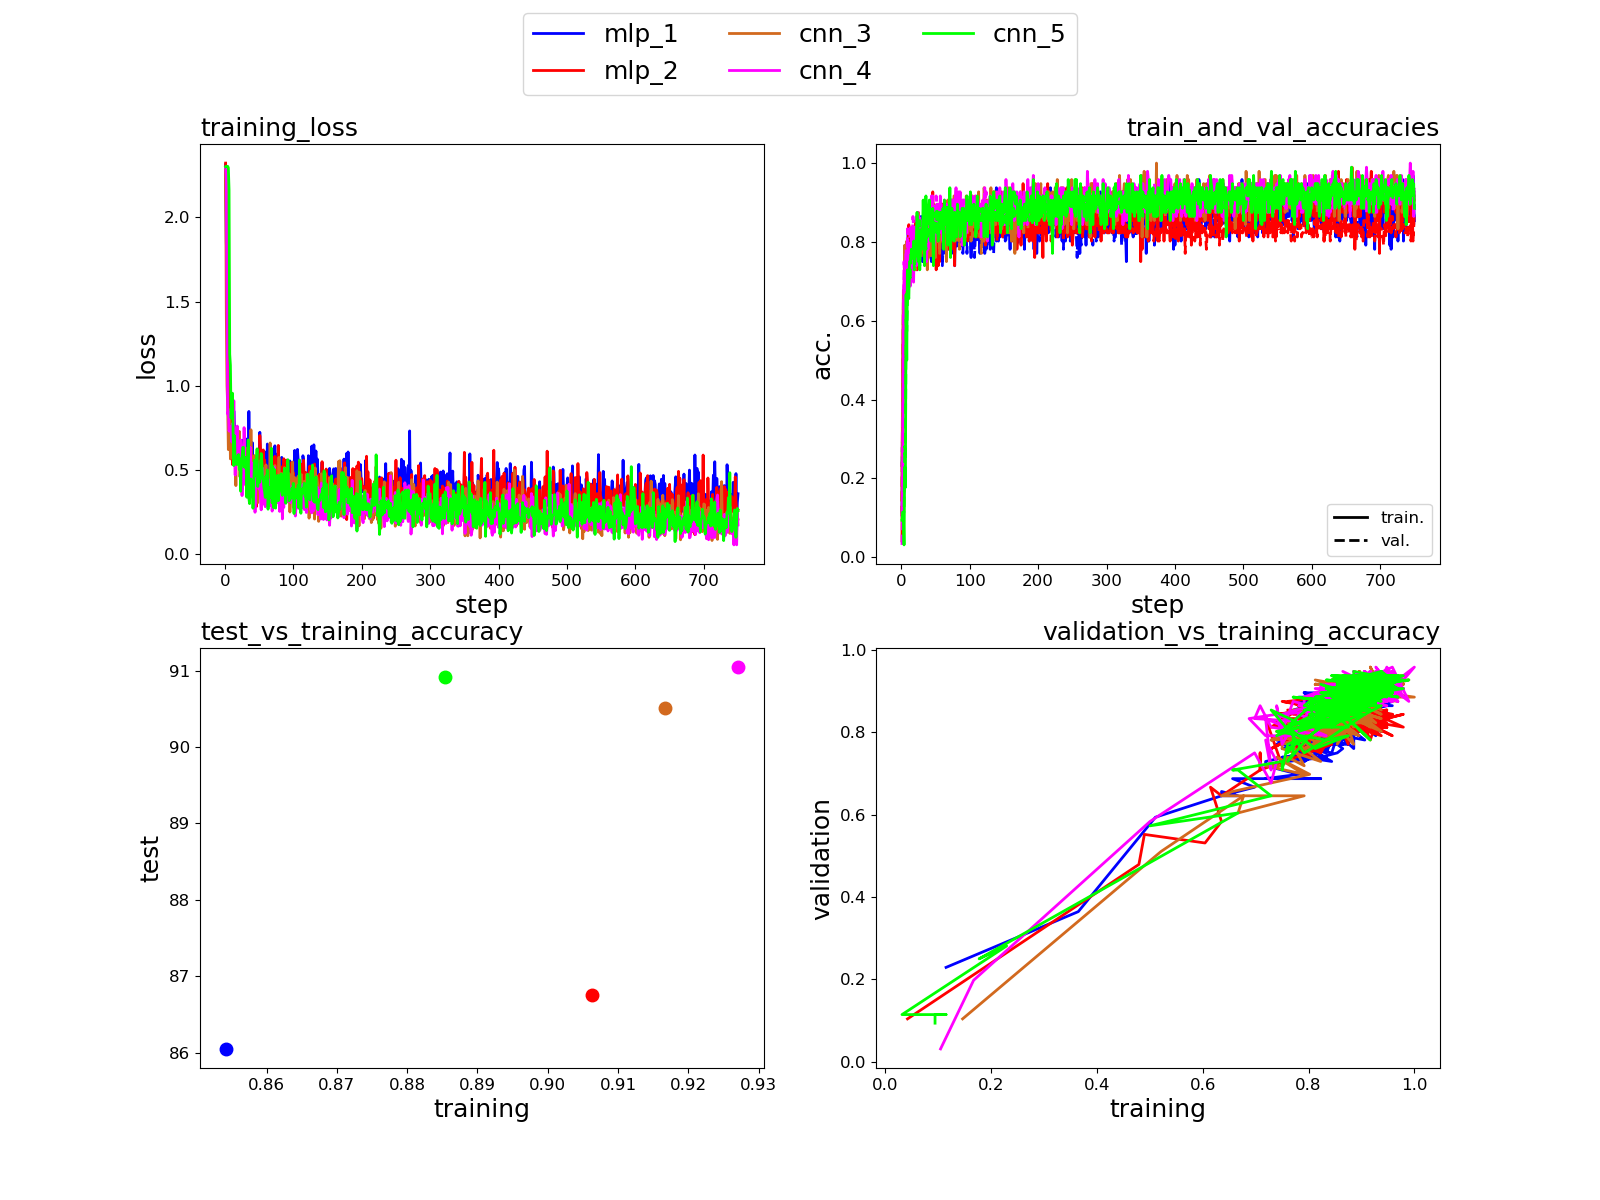
\includegraphics[width=1\textwidth]{figures/q3_results.png}
    \caption{Benchmark of five different architectures.}
    \label{Q3}
\end{figure}


\begin{figure}[htbp!]
    \begin{subfigure}{0.5\textwidth}
        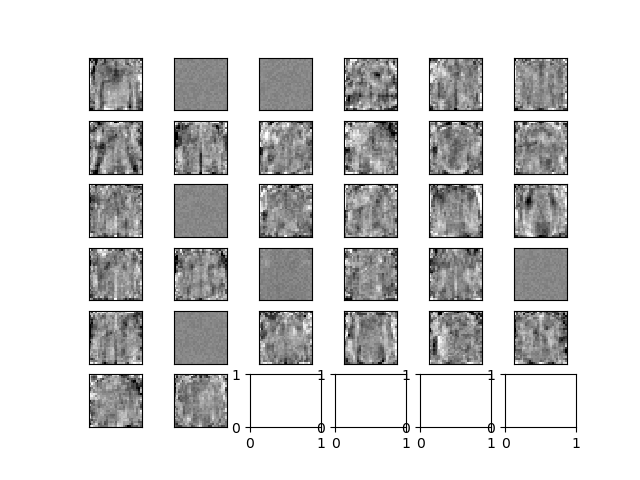
\includegraphics[width=\textwidth]{figures/weights_mlp_1.png}
        \caption{mlp 1}
    \end{subfigure}\hfill
    \begin{subfigure}{0.5\textwidth}
        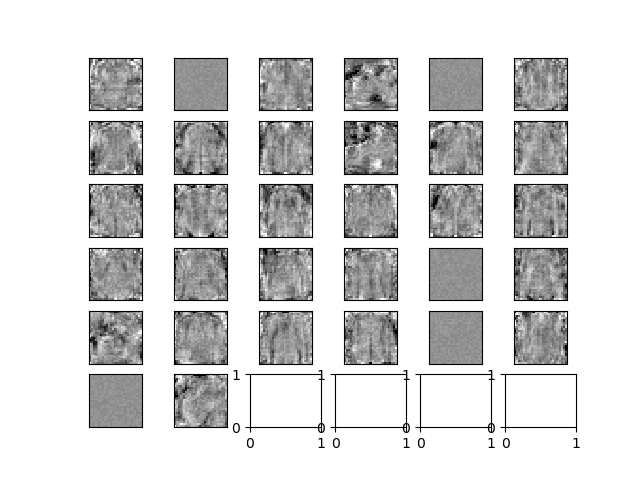
\includegraphics[width=\textwidth]{figures/weights_mlp_2.png}
        \caption{mlp 2}
    \end{subfigure}\vskip\baselineskip
    \begin{subfigure}{0.3\textwidth}
        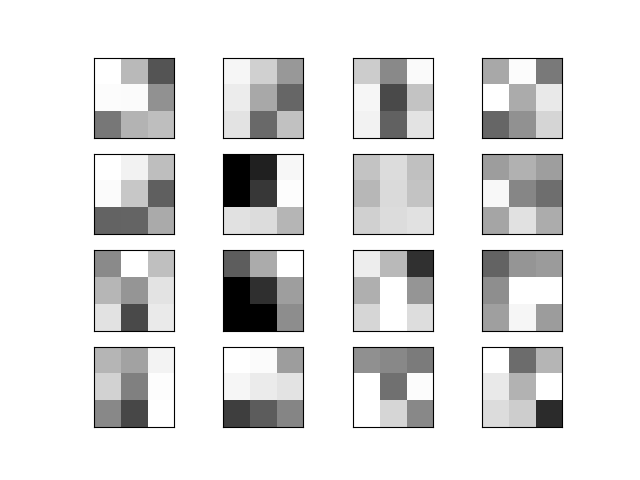
\includegraphics[width=\textwidth]{figures/weights_cnn_3.png}
        \caption{cnn 3}
    \end{subfigure}
    \hfill
    \begin{subfigure}{0.3\textwidth}
        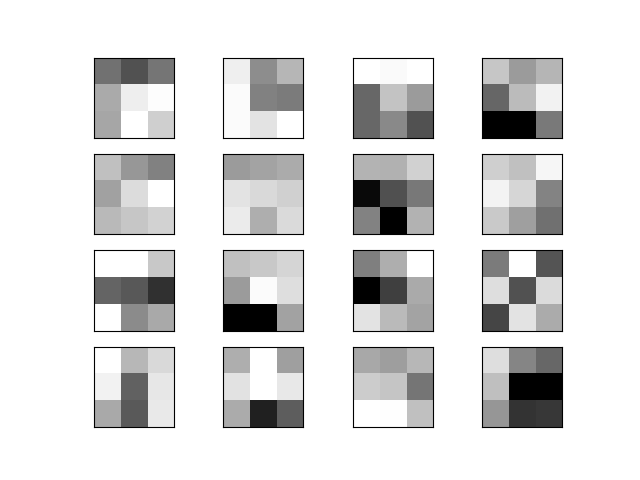
\includegraphics[width=\textwidth]{figures/weights_cnn_4.png}
        \caption{cnn 4}
    \end{subfigure}\hfill
    \begin{subfigure}{0.3\textwidth}
        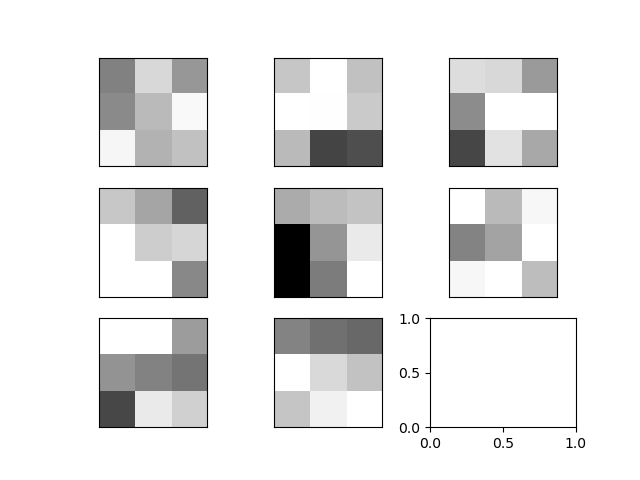
\includegraphics[width=\textwidth]{figures/weights_cnn_5.png}
        \caption{cnn 5}
    \end{subfigure}\hfill
    \caption{Weights of the first layers.}
    \label{fig:weights}
\end{figure}

\subsection{Question 3.2}


\textbf{1.}
\textbf{2.}
\textbf{3.}
\textbf{4.}
\textbf{5.}
\textbf{6.}
\textbf{7.}
\textbf{8.}
\textbf{9.}
\textbf{10.}


\section{Question 4}

\section{Question 5}



%--------------------------------------BIBLIOGRAFIA-------------------------------------------

\newpage
\section{References}
\nocite{*} 
\bibliographystyle{ieeetr}   
\bibliography{refs}     


\end{document}